\chapter{Theoretical background}\label{background}

In this chapter we will provide the necessary background for the user to understand the mechanisms used later in the paper. The description of the following systems is a brief introduction, intended to familiarize the reader with concepts that are fundamental for the methods presented.

Specifically, section \ref{sec:gzip} describes the functionality of the gzip compression method and the algorithms that it entails. Section \ref{sec:sameorigin} covers the same-origin policy that applies in the web application security model. In section \ref{sec:tls} we explain the Transport Layer Security, which is the main protocol used today to provide communications security over the Internet. Finally, in section \ref{sec:mitm} we describe attack methodologies in order for an adversary to perform a Man-in-the-middle attack, such as ARP spoofing and DNS poisoning.

\section{gzip}\label{sec:gzip}

gzip is a software application used for file compression and decompression. It is the most used encryption method on the Internet, integrated in protocols such as the Hypertext Transfer Protocol (HTTP), the Extensible Messaging and Presence Protocol (XMPP) and many more. Derivatives of gzip include the tar utility, which can extract .tar.gz files, as well as zlib, an abstraction of the DEFLATE algorithm in library form.\footnote{\url{https://en.wikipedia.org/wiki/Gzip}}

It is based on the DEFLATE algorithm, which is a combination of LZ77 and Huffman coding. DEFLATE could be described by the following encryption schema:

\begin{math}DEFLATE(m) = Huffman(LZ77(m))\end{math}

In the following sections we will briefly describe the functionality of both these compression algorithms.

\subsection{LZ77}
LZ77 is a lossless data compression algorithm published in paper by A. Lempel and J. Ziv in 1977. \cite{lz77} It achieves compression by replacing repeated occurences of data with references to a copy of that data existing earlier in the uncompressed data stream. The reference composes of a pair of numbers, the first of which represents the length of the repeated portion, while the second describes the distance backwards in the stream, until the beginning of the portion is met. In order to spot repeats, the protocol needs to keep track of some amount of the most recent data, specifically the 32 Kb latest. This data is held in a sliding window, so, in order for a portion of data to be compressed, the initial appearance of this repeated portion needs to have occurred at most 32 Kb up the data stream. Also, the minimum legth of a text to be compressed is 3 characters, while compressed text can also have literals as well as pointers.

Below you can see an example of a step-by-step execution of the algorithm for a specific text:

\begin{figure}[h!] \caption{First we get the plaintext to be compressed.} \centering 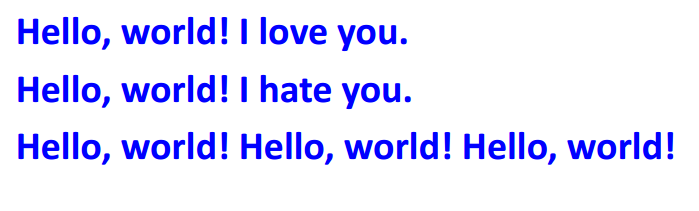
\includegraphics[width=0.5\textwidth]{diagrams/lz77_1.png}\end{figure}
\begin{figure}[h!] \caption{Compression starts with literal representation.} \centering 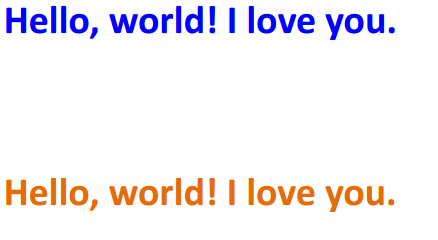
\includegraphics[width=0.35\textwidth]{diagrams/lz77_2.png}\end{figure}
\begin{figure}[h!] \caption{We then use a pointer at distance 26 and length 16.} \centering 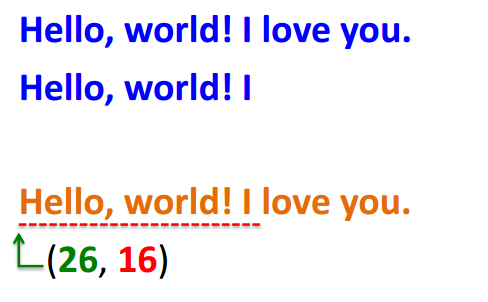
\includegraphics[width=0.35\textwidth]{diagrams/lz77_3.png}\end{figure}
\begin{figure}[h!] \caption{We continue with literal.} \centering 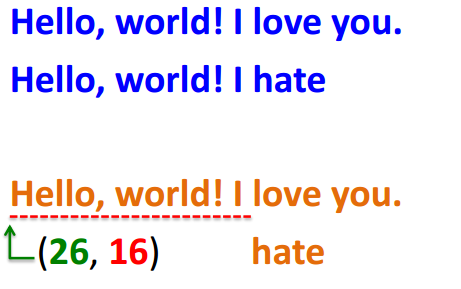
\includegraphics[width=0.35\textwidth]{diagrams/lz77_4.png}\end{figure}
\begin{figure}[h!] \caption{We use a pointer pointing to a pointer.} \centering 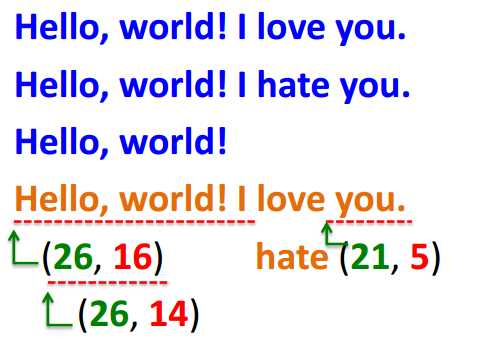
\includegraphics[width=0.35\textwidth]{diagrams/lz77_5.png}\end{figure}
\begin{figure}[h!] \caption{We then use a pointer pointing to a pointer pointing to a pointer.} \centering 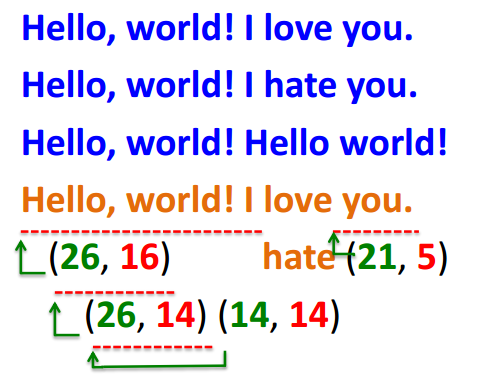
\includegraphics[width=0.35\textwidth]{diagrams/lz77_6.png}\end{figure}
\begin{figure}[h!] \caption{Finally, we use a pointer pointing to itself.} \centering 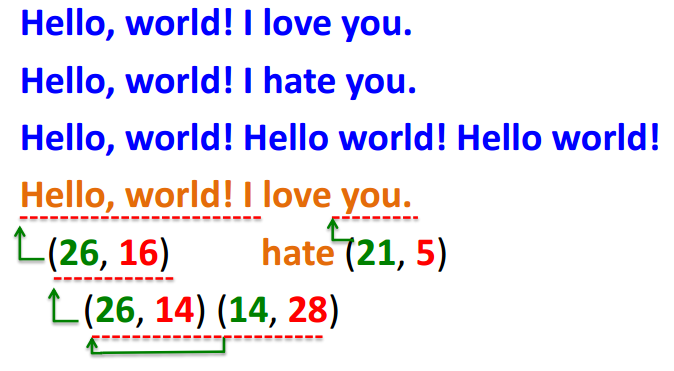
\includegraphics[width=0.5\textwidth]{diagrams/lz77_7.png}\end{figure}
